\documentclass[xcolor=table,handout]{beamer}
\setbeamertemplate{navigation symbols}{}

\usepackage{pgfpages}
\usepackage{adjustbox}
% \setbeameroption{show notes}
% \setbeameroption{show notes on second screen=right}

\usepackage{booktabs}
\usepackage{beamerthemeshadow}
\setbeamertemplate{caption}[numbered]
\setbeamerfont{caption}{size=\tiny}

\begin{document}

\title{Journal Club Presentation: Ocean Color}  
\author[K. Bellock, L. Chen, D. Durrance, A. Yen]{Kenneth Bellock, Leshi Chen, Danielle Durrance, Andrew Yen}
\titlegraphic{%
    \includegraphics[height=.37\textheight]{15_037}

    \tiny \textbf{Source:} \url{https://www.nasa.gov/press/2015/march/new-nasa-mission-to-study-ocean-color-airborne-particles-and-clouds}
}
\date{\vspace*{-2.5em}\par April 4, 2018} 

\section{Introduction}

\begin{frame}
  \titlepage{}
  \note{Assumptions:}
  \note[item]{TODO:\@ List assumptions.}
\end{frame}

\begin{frame}\frametitle{Table of contents}
  \tableofcontents{}
  \note[item]{A road map is a great thing to have.}
  \note[item]{A joke or reference to current events in common culture would be great here if the audience appears receptive.}
\end{frame} 

\begin{frame}\frametitle{Introduction} 
Ocean Color refers to the multi-colored ocean map products created from the measurements of chlorophyll by global satellites. The satellites, equipped with temporal scanners, collect water-leaving radiances of the Earth’s oceans.

Ocean color products are useful to gain insight of the physical and chemical processes occurring in Earth’s oceans. Chlorophyll concentration maps can be used for climate studies, measuring the salinity of oceans, estimating carbon levels of ocean regions, and studying phytoplankton species.

  \note[item]{TODO:\@ Write Introduction}
\end{frame}


\section{Article Summaries}

\begin{frame}\frametitle{Biospheric Primary Production During an ENSO Transition} 
\begin{description}
    \item[Authors] Michael J. Behrenfield, James T. Randerson, Charles R. McClain, Gene C. Feldman, Sietse O. Los, Compton J. Tucker, Paul G. Falkowski, Christopher B. Field, Robert Frouin, Wayne E. Esaias, Dorota D. Kolber, Nathan H. Pollack
    \item[Objectives] To compare the simultaneous ocean and land net primary production (NPP) responses to El Nino to La Nina transitions utilizing SeaWiFS measurements of chlorophyll concentration ($C_{sat}$) in the oceans and Normalized Difference Vegetation Index (NDVI) on land.
    \item[Methods] Characterization of global, 4-km resolution, monthly SeaWiFS $C_{sat}$ and NDVI data sensed between Septermber 1997 and August 2000, an El Nino to La Nina transition period.
\end{description}
  \note[item]{Include notes and talking points here.}
  \note[item]{There can be more than one note.}
\end{frame}

\begin{frame}\frametitle{Biospheric Primary Production During an ENSO Transition} 
\begin{description}
    \item[Findings] The greatest increases in ocean NPP were found in regions most impacted by El Nino-Sourthern Oscillation (ENSO). The figure on the following slide shows\ldots
    \item[A)] Average NPP for the La Nina Austral summer of December 1998 to February 1999
    \item[B)] Average NPP for the La Nina Boreal summer of June to August 1999
    \item[C)] Transition from El Nino to La Nina conditions
    \item[D)] Changes in NPP between two La Nina Boreal summers
\end{description}
\end{frame}

\begin{frame}\frametitle{Biospheric Primary Production During an ENSO Transition} 
    \begin{center}
        \includegraphics[width=\textwidth,height=0.8\textheight,keepaspectratio]{npp}
    \end{center}
  \note[item]{Pretty picture}
\end{frame}

\begin{frame}\frametitle{Performance of the MODIS semi-analytical ocean color algorithm for chlorophyll-a} 
\scriptsize
\begin{description}
    \item[Authors] K.L. Carder, F.R. Chen, J.P. Cannizzaro, J.W. Campbell, B.G. Mitchell
    \item[Objectives] Test effectiveness of MODIS semi-analytical algorithm (Chlor\_a\_3) against previous chlorophyll--a measurements from CZCS and SeaWiFS - particularly for high latitudes and regions with strong overturn, where chlorophyll-a (Chla) concentrations have been severely underestimated.
    
    \item[Methods] 
        \begin{itemize}
            \item Separation of the chlorophyll-specific phytoplankton absorption coefficient, $a^{\ast}_{ph}(\lambda)$ from gelbstoff/detritus for more accurate measures of chlorophyll-a.
            \item Previous algorithms for measuring chlorophyll concentration relied on the strong positive dependencies between the phytoplankton absorption coefficient at 440 nm and 675 nm, $a_{ph}(440, 675)$, and Chla. The SA algorithm is exceptional because it accommodates high degrees of variability of $a^{\ast}_{ph}(\lambda)$ in high-latitude/strong upwelling zones.
        \end{itemize}
\end{description}
\end{frame}

\begin{frame}\frametitle{Performance of the MODIS semi-analytical ocean color algorithm for chlorophyll-a} 
\scriptsize
\begin{description}
    \item[Findings]
        \begin{itemize}
            \item Chla can be accurately measured by empirical algorithms for $a_{ph}(675)$ $>$ 0.03 m-1, or 1.5 -2.0 mg/m3, but the semi-analytical algorithm is necessary for $a_{ph}(675)$ $<$ 0.03 m-1.
            \item near 1:1 relationship between SA modeled Chla and in situ Chla measurements, with significantly worse performance from modeled Chla using the empirical Chlor\_a\_2 algorithm (0.5:1, and 0.7:1 underestimations for two different study areas). 
            \item Chlor\_a\_2 and Chlor\_a\_3 both tend to agree with their estimations of Chla in equatorial waters, with the exception of zones of strong upwelling equatorial waters in the Eastern Pacific.
            \item The SA algorithm showed lower concentrations in chlorophyll-a than Chlor\_a\_2 in parts of the northern hemisphere because it was more effective at distinguishing between gelbstoff-rich runoff from northern rivers and ocean chlorophyll.
            \item One the most noticeable differences in Chla values is in high-latitude waters in the southern hemisphere during austral spring, where chlorophyll concentration in phytoplankton blooms was misrepresented by Chlor\_a\_2 because of chlorophyll packaging. 
        \end{itemize}
\end{description}

  \note[item]{Include notes and talking points here.}
  \note[item]{There can be more than one note.}
\end{frame}

\begin{frame}\frametitle{Performance of the MODIS semi-analytical ocean color algorithm for chlorophyll-a} 

  \note[item]{TODO:\@ Include a pretty picture.}
\end{frame}

\begin{frame}\frametitle{Decadal changes in global ocean chlorophyll} 
\begin{description}
    \item[Authors] Watson W. Gregg, Margarita E. Conkright
    \item[Objectives] The authors aim at finding decadal trends in global ocean chlorophyll between data obtained by CZCS (1979-1986) and those by SeaWiFS (1992– 2000).
    \item[Methods]
        \begin{itemize}
            \item Chlorophyll data from CZCS and SeaWiFS are combined for reanalysis at 1° spatial resolution. 
            \item To increase compatibility and to reduce residual errors, both archives are blended with in situ data. 
        \end{itemize}
\end{description}

  \note[item]{Include notes and talking points here.}
  \note[item]{There can be more than one note.}
\end{frame}

\begin{frame}\frametitle{Decadal changes in global ocean chlorophyll} 
\begin{description}
    \item[Findings] 
        \begin{itemize}
            \item There is large similarity in the global spatial distributions and seasonal variability between the two chlorophyll archives.  
            \item On average, the global ocean chlorophyll has decreased from the CZCS archive to the SeaWiFS by 6\%, and changes are mainly observed in summer and autumn.  
            \item Reductions in North Pacific and North Atlantics in summer are mainly caused by reduced wind stresses and warmer sea surface temperature (SST).  
            \item Regional meteorological events, such as PDP and ENSO have contributed to the changes in global ocean chlorophyll. 
        \end{itemize}
\end{description}
  \note[item]{Include a note if needed.}
\end{frame}

\begin{frame}\frametitle{Decadal changes in global ocean chlorophyll} 
    \hfill
    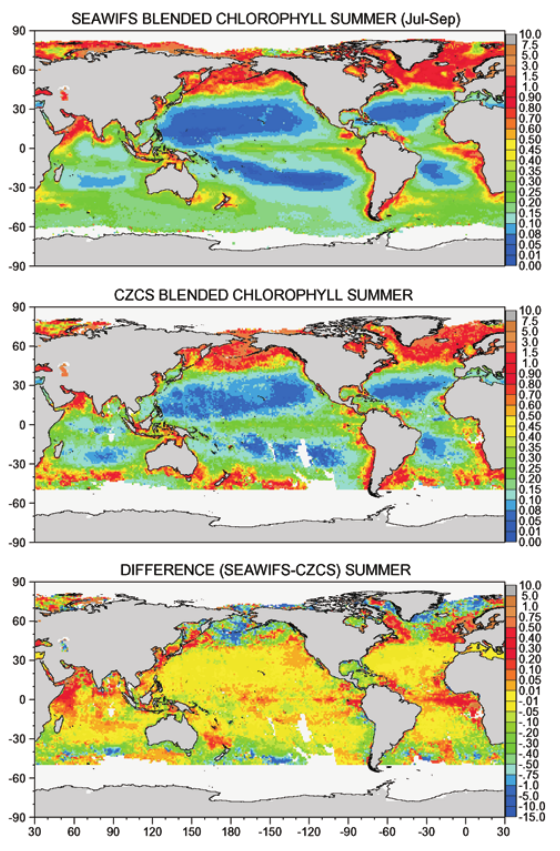
\includegraphics[width=\textwidth,height=0.8\textheight,keepaspectratio]{gregg1}
    \hfill
    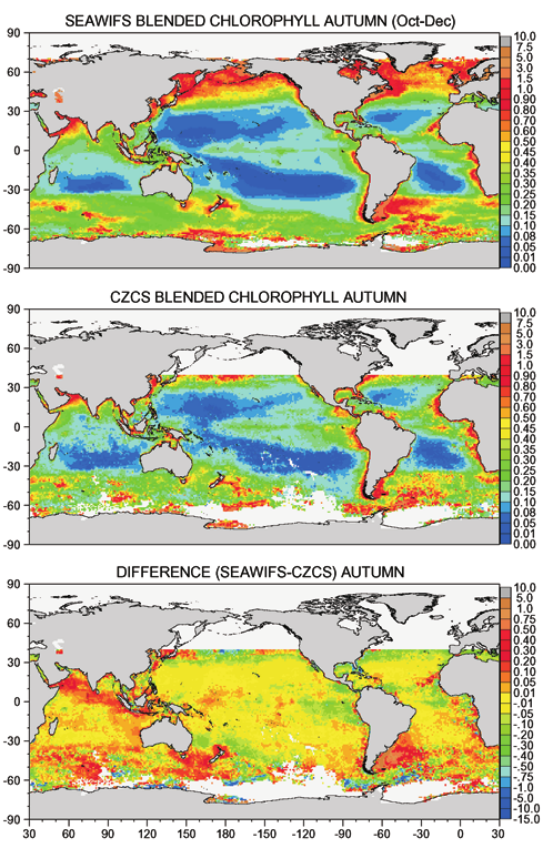
\includegraphics[width=\textwidth,height=0.8\textheight,keepaspectratio]{gregg2}
    \hfill
  \note[item]{Pretty pictures}
\end{frame}

\begin{frame}\frametitle{Corrections to the Calibration of MODIS Aqua Ocean Color Bands Derived From SeaWiFS Data} 
\begin{description}
    \item[Authors] Gerhard Meister, Bryan A. Franz, Ewa J. Kwiatkowska, Charles R. McClain
    \item[Summary] \scriptsize A new calibration method was needed to correct a problem affecting the Moderate Resolution Imaging Spectroradiometer, MODIS Aqua’s, ability to provide accurate ocean color data. The system uses bands 8-14 to detect water leaving radiances from the Earth’s surface. The problem affected temporal information collected for wavelengths between 412-443 nm. Prior to the calibration issues, the MODIS Calibration and Support Team (MCST) used onboard calibrators and lunar irradiances to sufficiently calibrate the MODIS systems. Now, the calibration methods are based on the Ocean Biology Processing Group’s (OBPG) calibration solution for MODIS Terra, which experienced a similar problem. In this method, the MODIS system is cross-calibrated with SeaWiFS to recharacterize the data to correct for the temporal trend error. Now, ocean color data is made with SeaWiFS and MODIS Aqua data merged together. Each data set is processed on its own and then reconfigured.
\end{description}

  \note[item]{Include notes and talking points here.}
  \note[item]{There can be more than one note.}
\end{frame}

\begin{frame}\frametitle{Corrections to the Calibration of MODIS Aqua Ocean Color Bands Derived From SeaWiFS Data} 


\begin{columns}
\begin{column}{0.5\textwidth}
    \begin{center}
    \textbf{\scriptsize SEAWIFS SWATHS}
    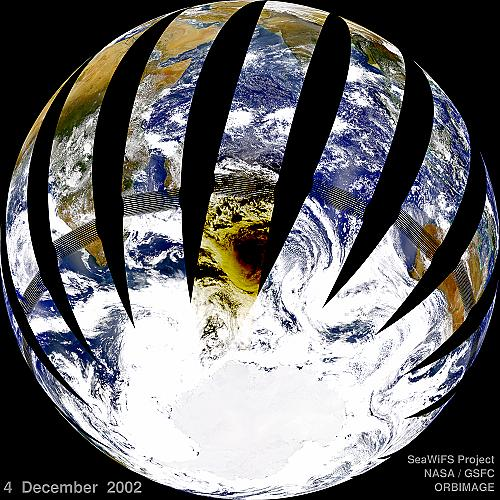
\includegraphics[width=\textwidth,height=0.8\textheight,keepaspectratio]{N7Pw7r}

    \tiny \textbf{Source:} \url{http://epod.typepad.com/.a/6a0105371bb32c970b0115714d7c00970c-500wi}
    \end{center}
\end{column}
\begin{column}{0.5\textwidth}  %%<--- here
    \begin{center}
    \textbf{\scriptsize MODIS AQUA PREDICTED PATHS}
    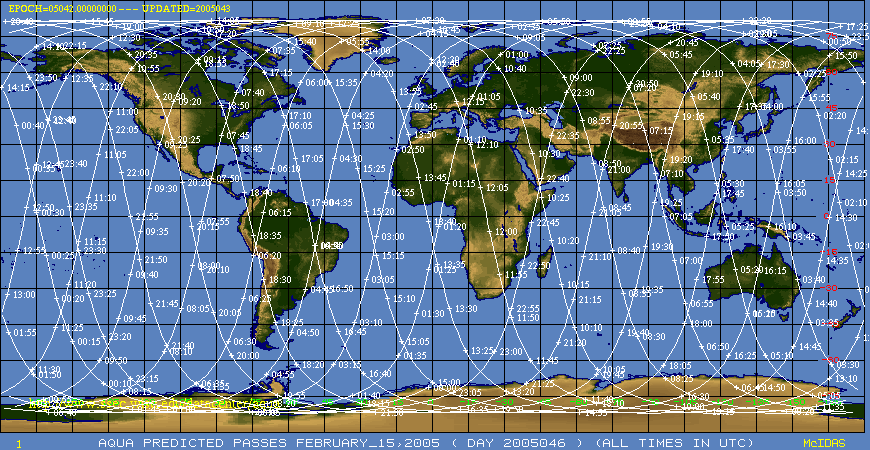
\includegraphics[width=\textwidth,height=0.8\textheight,keepaspectratio]{kVvOUr}

    \tiny \textbf{Source:} \url{https://nsidc.org/sites/nsidc.org/files/aqua_tracks.20050215.gif}
    \end{center}
\end{column}
\end{columns}

\end{frame}


\section{Summary and Conclusion}

\begin{frame}\frametitle{Summary} 

  \note[item] These studies on ocean color discuss the evolution of chlorophyll-a measurements through advancements in remote sensing capabilities stemming from:
  \begin{itemize}
    \item Refining instrument calibration and assimilating datasets for long-term reanalysis.
    \item Better understanding of the effects of inter-annual and irregular climate phenomena on NPP and Phytoplankton absorption.
    \item Redesign of Chlorophyll-a algorithms for distinguishing between different absorptive ocean water constituents. 
  \end{itemize}
  All of these advancements have profound implications for a more clear understanding of the ocean's contribution to the Earth's carbon cycle.
\end{frame}

\begin{frame}\frametitle{Conclusion} 
Ocean color is best sensed by global satellites to fully capture all available data for accurate analysis. Calculations are performed to compare differing levels of chlorophyll in the Earth’s oceans in different seasons or years. The chlorophyll levels offer insight on the non-water contents of the oceans to monitor for potentially harmful changes. Chlorophyll levels are affected primarily by water temperature, water currents, and nutrient levels. Significant shifts in chlorophyll concentrations can indicate the occurrence of certain events. Ocean color mapping is a useful tool to find the source of problematic events so problem solving can begin. 
  \note[item]{TODO:\@ Write Conclusion}
\end{frame}


\end{document}
